\documentclass[ignorenonframetext,]{beamer}
\usetheme{default}
\usecolortheme{rose}
\usepackage{amssymb,amsmath}
\usepackage{ifxetex,ifluatex}
\usepackage{fixltx2e} % provides \textsubscript
\ifxetex
  \usepackage{fontspec,xltxtra,xunicode}
  \defaultfontfeatures{Mapping=tex-text,Scale=MatchLowercase}
\else
  \ifluatex
    \usepackage{fontspec}
    \defaultfontfeatures{Mapping=tex-text,Scale=MatchLowercase}
  \else
    \usepackage[utf8]{inputenc}
  \fi
\fi
\usepackage{color}
\usepackage{fancyvrb}
\DefineShortVerb[commandchars=\\\{\}]{\|}
\DefineVerbatimEnvironment{Highlighting}{Verbatim}{commandchars=\\\{\}}
% Add ',fontsize=\small' for more characters per line
\newenvironment{Shaded}{}{}
\newcommand{\KeywordTok}[1]{\textcolor[rgb]{0.00,0.44,0.13}{\textbf{{#1}}}}
\newcommand{\DataTypeTok}[1]{\textcolor[rgb]{0.56,0.13,0.00}{{#1}}}
\newcommand{\DecValTok}[1]{\textcolor[rgb]{0.25,0.63,0.44}{{#1}}}
\newcommand{\BaseNTok}[1]{\textcolor[rgb]{0.25,0.63,0.44}{{#1}}}
\newcommand{\FloatTok}[1]{\textcolor[rgb]{0.25,0.63,0.44}{{#1}}}
\newcommand{\CharTok}[1]{\textcolor[rgb]{0.25,0.44,0.63}{{#1}}}
\newcommand{\StringTok}[1]{\textcolor[rgb]{0.25,0.44,0.63}{{#1}}}
\newcommand{\CommentTok}[1]{\textcolor[rgb]{0.38,0.63,0.69}{\textit{{#1}}}}
\newcommand{\OtherTok}[1]{\textcolor[rgb]{0.00,0.44,0.13}{{#1}}}
\newcommand{\AlertTok}[1]{\textcolor[rgb]{1.00,0.00,0.00}{\textbf{{#1}}}}
\newcommand{\FunctionTok}[1]{\textcolor[rgb]{0.02,0.16,0.49}{{#1}}}
\newcommand{\RegionMarkerTok}[1]{{#1}}
\newcommand{\ErrorTok}[1]{\textcolor[rgb]{1.00,0.00,0.00}{\textbf{{#1}}}}
\newcommand{\NormalTok}[1]{{#1}}
\usepackage{enumerate}
\usepackage{url}
% Comment these out if you don't want a slide with just the
% part/section/subsection/subsubsection title:
\AtBeginPart{\frame{\partpage}}
\AtBeginSection{\frame{\sectionpage}}
\AtBeginSubsection{\frame{\subsectionpage}}
\AtBeginSubsubsection{\frame{\subsubsectionpage}}
\setlength{\parindent}{0pt}
\setlength{\parskip}{6pt plus 2pt minus 1pt}
\setlength{\emergencystretch}{3em}  % prevent overfull lines
\setcounter{secnumdepth}{0}

\title{MUSI3620/40 Music Technology}
\author{Processing 1 - Introduction}
\date{Alex McLean}

\begin{document}
\frame{\titlepage}

\begin{frame}\frametitle{Processing}


\includegraphics[width=0.1\textwidth]{../images/processing2-logo.jpg}

\begin{itemize}
\item
  Free/open source project
\item
  Initiated by Casey Reas and Ben Fry in 2005
\item
  For learning programming in visual context
\item
  Based on Java, but simplified
\item
  Sketchbook metaphor
\end{itemize}

\end{frame}

\begin{frame}\frametitle{On-line documentation}

\begin{center}

\includegraphics[width=0.5\textwidth]{../images/processingorg.png}

\url{https://processing.org/}
\end{center}

\begin{itemize}
\item
  Reference, Tutorials, Forum
\item
  Off-line from UI:

  \begin{itemize}
  \item
    Help -\textgreater{} reference
  \item
    Right click on code -\textgreater{} find in reference
  \end{itemize}
\end{itemize}

\end{frame}

\begin{frame}[fragile]\frametitle{Further reading}


\includegraphics[width=0.4\textwidth]{../images/learningprocessing.jpg}

Video lectures: \url{http://icm.shiffman.net/}

More books: \url{http://processing.org/books/}

\end{frame}

\begin{frame}\frametitle{Open processing}

\begin{center}
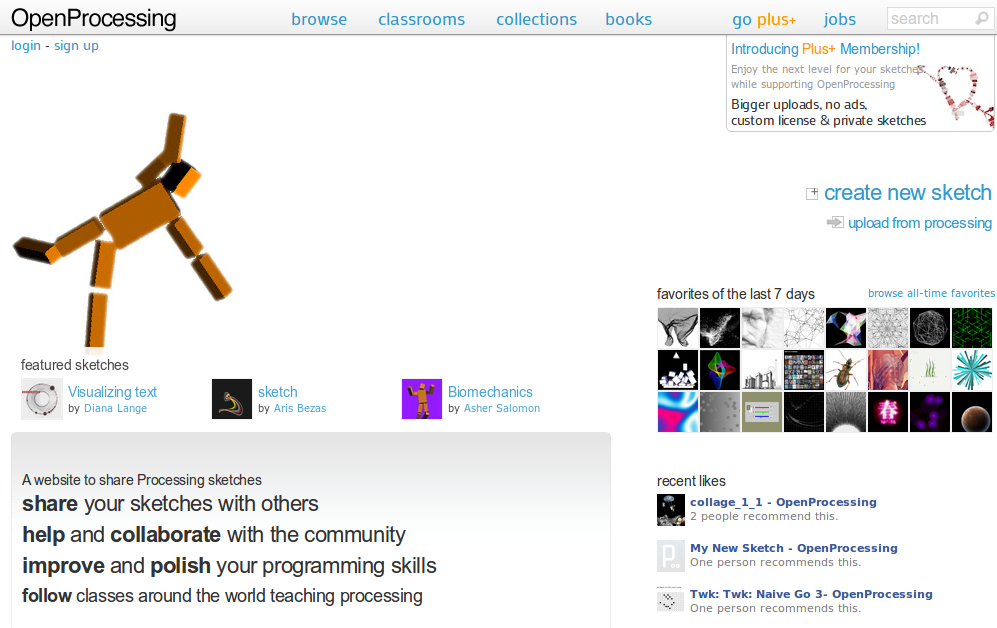
\includegraphics[width=0.5\textwidth]{../images/openprocessing.png}

\url{https://openprocessing.org/}
\end{center}

\end{frame}

\begin{frame}\frametitle{Examples}

File -\textgreater{} Examples

\begin{center}
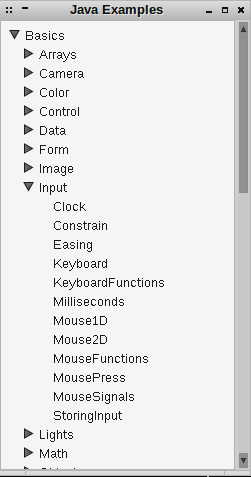
\includegraphics[width=0.3\textwidth]{../images/examples.png}
\end{center}

\end{frame}

\begin{frame}\frametitle{Lets get programming}

\begin{itemize}
\item
  Draw some shapes
\item
  Play a sound
\end{itemize}

\end{frame}

\begin{frame}[fragile]\frametitle{Draw a circle}

Use the \href{http://processing.org/reference/ellipse\_.html}{ellipse}
function call

\begin{Shaded}
\begin{Highlighting}[]
\CommentTok{// x, y, width, height}
\FunctionTok{ellipse}\NormalTok{(}\DecValTok{10}\NormalTok{,}\DecValTok{10}\NormalTok{,}\DecValTok{10}\NormalTok{,}\DecValTok{10}\NormalTok{);}
\end{Highlighting}
\end{Shaded}

\end{frame}

\begin{frame}[fragile]\frametitle{Draw a square}

Use the \href{http://processing.org/reference/rect\_.html}{rect}
function call

\begin{Shaded}
\begin{Highlighting}[]
\CommentTok{// x, y, width, height}
\FunctionTok{rect}\NormalTok{(}\DecValTok{30}\NormalTok{,}\DecValTok{30}\NormalTok{,}\DecValTok{10}\NormalTok{,}\DecValTok{10}\NormalTok{);}
\end{Highlighting}
\end{Shaded}

\end{frame}

\begin{frame}[fragile]\frametitle{Change the brush colour}

Specify colour as red, green and blue components, from 0 to 255.

\begin{Shaded}
\begin{Highlighting}[]
\FunctionTok{stroke}\NormalTok{(}\DecValTok{0}\NormalTok{,}\DecValTok{0}\NormalTok{,}\DecValTok{0}\NormalTok{);}

\FunctionTok{fill}\NormalTok{(}\DecValTok{255}\NormalTok{,}\DecValTok{0}\NormalTok{,}\DecValTok{0}\NormalTok{);}
\FunctionTok{ellipse}\NormalTok{(}\DecValTok{10}\NormalTok{,}\DecValTok{10}\NormalTok{,}\DecValTok{10}\NormalTok{,}\DecValTok{10}\NormalTok{);}

\FunctionTok{fill}\NormalTok{(}\DecValTok{0}\NormalTok{,}\DecValTok{255}\NormalTok{,}\DecValTok{0}\NormalTok{);}
\FunctionTok{rect}\NormalTok{(}\DecValTok{30}\NormalTok{,}\DecValTok{30}\NormalTok{,}\DecValTok{10}\NormalTok{,}\DecValTok{10}\NormalTok{);}

\FunctionTok{fill}\NormalTok{(}\DecValTok{0}\NormalTok{,}\DecValTok{0}\NormalTok{,}\DecValTok{255}\NormalTok{);}
\CommentTok{// x1, y1, x2, y2, x3, y3}
\FunctionTok{triangle}\NormalTok{(}\DecValTok{40}\NormalTok{,}\DecValTok{40}\NormalTok{,}\DecValTok{50}\NormalTok{,}\DecValTok{40}\NormalTok{,}\DecValTok{55}\NormalTok{,}\DecValTok{45}\NormalTok{);}

\FunctionTok{stroke}\NormalTok{(}\DecValTok{0}\NormalTok{,}\DecValTok{0}\NormalTok{,}\DecValTok{255}\NormalTok{);}
\FunctionTok{line}\NormalTok{(}\DecValTok{0}\NormalTok{,}\DecValTok{0}\NormalTok{,}\DecValTok{50}\NormalTok{,}\DecValTok{50}\NormalTok{);}
\end{Highlighting}
\end{Shaded}

\end{frame}

\begin{frame}[fragile]\frametitle{Exercise 1}

Draw a face (or something) using fill, stroke, ellipse, rect and line.

Reminder:

\begin{Shaded}
\begin{Highlighting}[]
\CommentTok{// red, green, blue component from 0 to 255}
\FunctionTok{fill}\NormalTok{(}\DecValTok{0}\NormalTok{, }\DecValTok{255}\NormalTok{, }\DecValTok{255}\NormalTok{);}
\CommentTok{// Same, but for line colour (e.g. around a shape)}
\FunctionTok{stroke}\NormalTok{(}\DecValTok{255}\NormalTok{, }\DecValTok{0}\NormalTok{, }\DecValTok{255}\NormalTok{);}

\CommentTok{// x, y, width, height in pixels}
\FunctionTok{ellipse}\NormalTok{(}\DecValTok{10}\NormalTok{, }\DecValTok{10}\NormalTok{, }\DecValTok{10}\NormalTok{, }\DecValTok{10}\NormalTok{);}

\CommentTok{// same as ellipse}
\FunctionTok{rect}\NormalTok{(}\DecValTok{20}\NormalTok{, }\DecValTok{20}\NormalTok{, }\DecValTok{10}\NormalTok{, }\DecValTok{10}\NormalTok{);}

\CommentTok{// fromX, fromY, toX, toY}
\FunctionTok{line}\NormalTok{(}\DecValTok{40}\NormalTok{, }\DecValTok{40}\NormalTok{, }\DecValTok{50}\NormalTok{, }\DecValTok{50}\NormalTok{);}
\end{Highlighting}
\end{Shaded}

\end{frame}

\begin{frame}[fragile]\frametitle{Loops - Draw ten squares}

\begin{Shaded}
\begin{Highlighting}[]
\DataTypeTok{int} \NormalTok{count = }\DecValTok{0}\NormalTok{;}
\KeywordTok{while} \NormalTok{(count < }\DecValTok{10}\NormalTok{) \{}
  \FunctionTok{fill}\NormalTok{((}\DecValTok{255}\NormalTok{/}\DecValTok{10}\NormalTok{) * count, }\DecValTok{255}\NormalTok{, }\DecValTok{0}\NormalTok{);}
  \FunctionTok{rect}\NormalTok{(count * }\DecValTok{10}\NormalTok{, }\DecValTok{10}\NormalTok{, }\DecValTok{10}\NormalTok{, }\DecValTok{10}\NormalTok{);}
  \CommentTok{// add 1 to count}
  \NormalTok{count = count + }\DecValTok{1}\NormalTok{;}
\NormalTok{\} }
\end{Highlighting}
\end{Shaded}

or

\begin{Shaded}
\begin{Highlighting}[]
\KeywordTok{for} \NormalTok{(}\DataTypeTok{int} \NormalTok{count = }\DecValTok{0}\NormalTok{; count < }\DecValTok{10}\NormalTok{; count++) \{}
  \FunctionTok{fill}\NormalTok{((}\DecValTok{255}\NormalTok{/}\DecValTok{10}\NormalTok{) * count, }\DecValTok{255}\NormalTok{, }\DecValTok{0}\NormalTok{);}
  \FunctionTok{rect}\NormalTok{(count * }\DecValTok{10}\NormalTok{, }\DecValTok{10}\NormalTok{, }\DecValTok{10}\NormalTok{, }\DecValTok{10}\NormalTok{);}
\NormalTok{\} }
\end{Highlighting}
\end{Shaded}

\end{frame}

\begin{frame}[fragile]\frametitle{Exercise 2: Make a sound}

Add the minim library to your sketch: (Sketch -\textgreater{} Import
library -\textgreater{} minim)

Download sound from \url{http://is.gd/kickdrum}

Add the sound to your sketch with Sketch -\textgreater{} Add file

\begin{Shaded}
\begin{Highlighting}[]
\CommentTok{// Initialise audio}
\NormalTok{Minim minim = }\KeywordTok{new} \FunctionTok{Minim}\NormalTok{(}\KeywordTok{this}\NormalTok{);}

\CommentTok{// Prepare a sound}
\NormalTok{AudioSample kick = minim.}\FunctionTok{loadSample}\NormalTok{(}\StringTok{"kick.wav"}\NormalTok{);}

\CommentTok{// Trigger the sound}
\NormalTok{kick.}\FunctionTok{trigger}\NormalTok{();}
\end{Highlighting}
\end{Shaded}

\end{frame}

\begin{frame}[fragile]\frametitle{Animation the Processing way}

Follows code in \texttt{setup()} once, and then in \texttt{draw()} every
frame.

\begin{Shaded}
\begin{Highlighting}[]
\CommentTok{// global variables}
\NormalTok{AudioSample kick;}

\DataTypeTok{void} \FunctionTok{setup}\NormalTok{() \{}
  \CommentTok{// make the canvas a bit bigger}
  \FunctionTok{size}\NormalTok{(}\DecValTok{300}\NormalTok{,}\DecValTok{300}\NormalTok{);}
  \NormalTok{Minim minim = }\KeywordTok{new} \FunctionTok{Minim}\NormalTok{(}\KeywordTok{this}\NormalTok{);}
  \NormalTok{kick = minim.}\FunctionTok{loadSample}\NormalTok{(}\StringTok{"kick.wav"}\NormalTok{);}
  \CommentTok{// follow draw() two times every second}
  \FunctionTok{frameRate}\NormalTok{(}\DecValTok{2}\NormalTok{);}
\NormalTok{\}}

\DataTypeTok{void} \FunctionTok{draw}\NormalTok{() \{}
  \FunctionTok{ellipse}\NormalTok{(}\FunctionTok{random}\NormalTok{(width),}\FunctionTok{random}\NormalTok{(height),}\DecValTok{10}\NormalTok{,}\DecValTok{10}\NormalTok{);}
  \NormalTok{kick.}\FunctionTok{trigger}\NormalTok{();}
\NormalTok{\}}
\end{Highlighting}
\end{Shaded}

\end{frame}

\begin{frame}[fragile]\frametitle{Exercise 3 - Movement}

\begin{Shaded}
\begin{Highlighting}[]
\CommentTok{// global variables}
\DataTypeTok{float} \NormalTok{bally = }\DecValTok{0}\NormalTok{;}
\DataTypeTok{float} \NormalTok{ballx = }\DecValTok{150}\NormalTok{;}

\DataTypeTok{void} \FunctionTok{setup}\NormalTok{() \{}
  \CommentTok{// make the canvas a bit bigger}
  \FunctionTok{size}\NormalTok{(}\DecValTok{300}\NormalTok{,}\DecValTok{300}\NormalTok{);}
\NormalTok{\}}

\DataTypeTok{void} \FunctionTok{draw}\NormalTok{() \{}
  \FunctionTok{ellipse}\NormalTok{(ballx,bally,}\DecValTok{10}\NormalTok{,}\DecValTok{10}\NormalTok{);}
\NormalTok{\}}
\end{Highlighting}
\end{Shaded}

\begin{enumerate}[1.]
\item
  Make the shape move

  \begin{itemize}
  \item
    Add another global variable that stores the speed of the shape
  \item
    Add \texttt{speed} to \texttt{bally} every frame (i.e.~within
    \texttt{draw()})
  \end{itemize}
\end{enumerate}

\end{frame}

\begin{frame}[fragile]\frametitle{Exercise 3 - Movement}

\begin{enumerate}[1.]
\setcounter{enumi}{1}
\item
  Make the shape bounce off the edges of the sketch and make a sound

  \begin{itemize}
  \item
    have an \texttt{if} statement that tests whether
    \texttt{bally \textgreater{} height}
  \item
    when that is true, play a sound and invert \texttt{speed}, (i.e.~set
    \texttt{speed = 0 - speed})
  \item
    do something similar for the top of the sketch (i.e.~when
    \texttt{bally} \textless{} 0)
  \item
    add the code to load a sound in \texttt{setup()}, and have a bounce
    trigger it in \texttt{draw()}
  \end{itemize}
\item
  Challenges: have multiple shapes, or add gravity effect.
\item
  Challenge question: Could we replace the \texttt{float} variables with
  \texttt{int} variables? What is the advantage of either?
\end{enumerate}

\end{frame}

\end{document}
